\section{Methodology}
\cref{subsec:1} introduces XX.
\cref{subsec:2} describes XX.
\cref{subsec:3} introduces XX.
\cref{subsec:4} describes XX.
\cref{subsec:5} describes XX.
%-------------------------------------------------------------------------
\subsection{Problem formulation}
\label{subsec:1}
\lipsum[1]
\begin{equation}
  \begin{cases}
  D = \{(I_i, P_i, T_i); i=1,2,\ldots,N\} \\
  P_i \in \{\text{A,B,C}\} \\
  T_i = MODEL(I_i, P_i), \quad i=1,2,\ldots,N \\
  \end{cases}
  \label{eq:1}
\end{equation}
\lipsum[4]
%-------------------------------------------------------------------------
\subsection{wdada wad fawefa}
\label{subsec:2}
\lipsum[4]

%-------------------------------------------------------------------------
\subsubsection{Podaiojndoa awed jmp}
\lipsum[4]
{\bf Wda wdgr gyuykjy:} \lipsum[1]

{\bf iojicbyu ujie:} \lipsum[1]
%-------------------------------------------------------------------------
\subsubsection{Oftwd r wfda }
\lipsum[4]

\begin{algorithm}[!hbp]
	\caption{daw da fghgrt s}
    \label{sdms}
    \begin{algorithmic}
      \REQUIRE dwa : $O:\{\theta_i, \rho_i, \vec p_i=(x_i, y_i) | i = 1,2,...,n\}$
        \STATE wad  $O$: $\mu \gets \frac{\sum_{i=1}^{n} \rho_i}{n}$ 
        \STATE wa  $O$: $\sigma^2 \gets \mu \frac{\sum_{i=1}^{n} (\rho_i - \mu)^2}{n-1}$  
        \STATE urtrhh:  $r = \mu+ \alpha \times \sigma$
        \STATE erwww: $\mathcal{D}:\{d_i = e^{-\frac{(\rho_i - r)^2}{2\sigma^2} }| i = 1,2,...,n\}$
        \STATE turtyhr: $x_s = \frac{\sum_{i=1}^{n} \omega_i x_i}{\sum_{i=1}^{n}\omega_i}$; $y_s = \frac{\sum_{i=1}^{n} \omega_i y_i}{\sum_{i=1}^{n}\omega_i}$
        \STATE 3wrwrf: $\vec p_u = (x_u, y_u)$, \\
              \hspace{2em}where: $x_u = \frac{x_s}{\sqrt{{x_s}^2 + {y_s}^2}}$; $y_u = \frac{y_s}{\sqrt{{x_s}^2 + {y_s}^2}}$
        \STATE w3rwrrwr: $\vec f_i = (1-d_i)\times \vec p_i + d_i \rho_i \times \vec p_u$
        \ENSURE 3rwrw: $O:\{\vec f_i | i = 1,2,...,n\}$
    \end{algorithmic}
\end{algorithm}
In \cref{sdms}, w3rwf. 
The \( \alpha \) waed okopfs. 
The \( \omega_i \) 3wrw3rw. 



\subsection{okpawdiodaw}
\label{subsec:4}
\lipsum[4]

\begin{figure}[H]
  \centering
  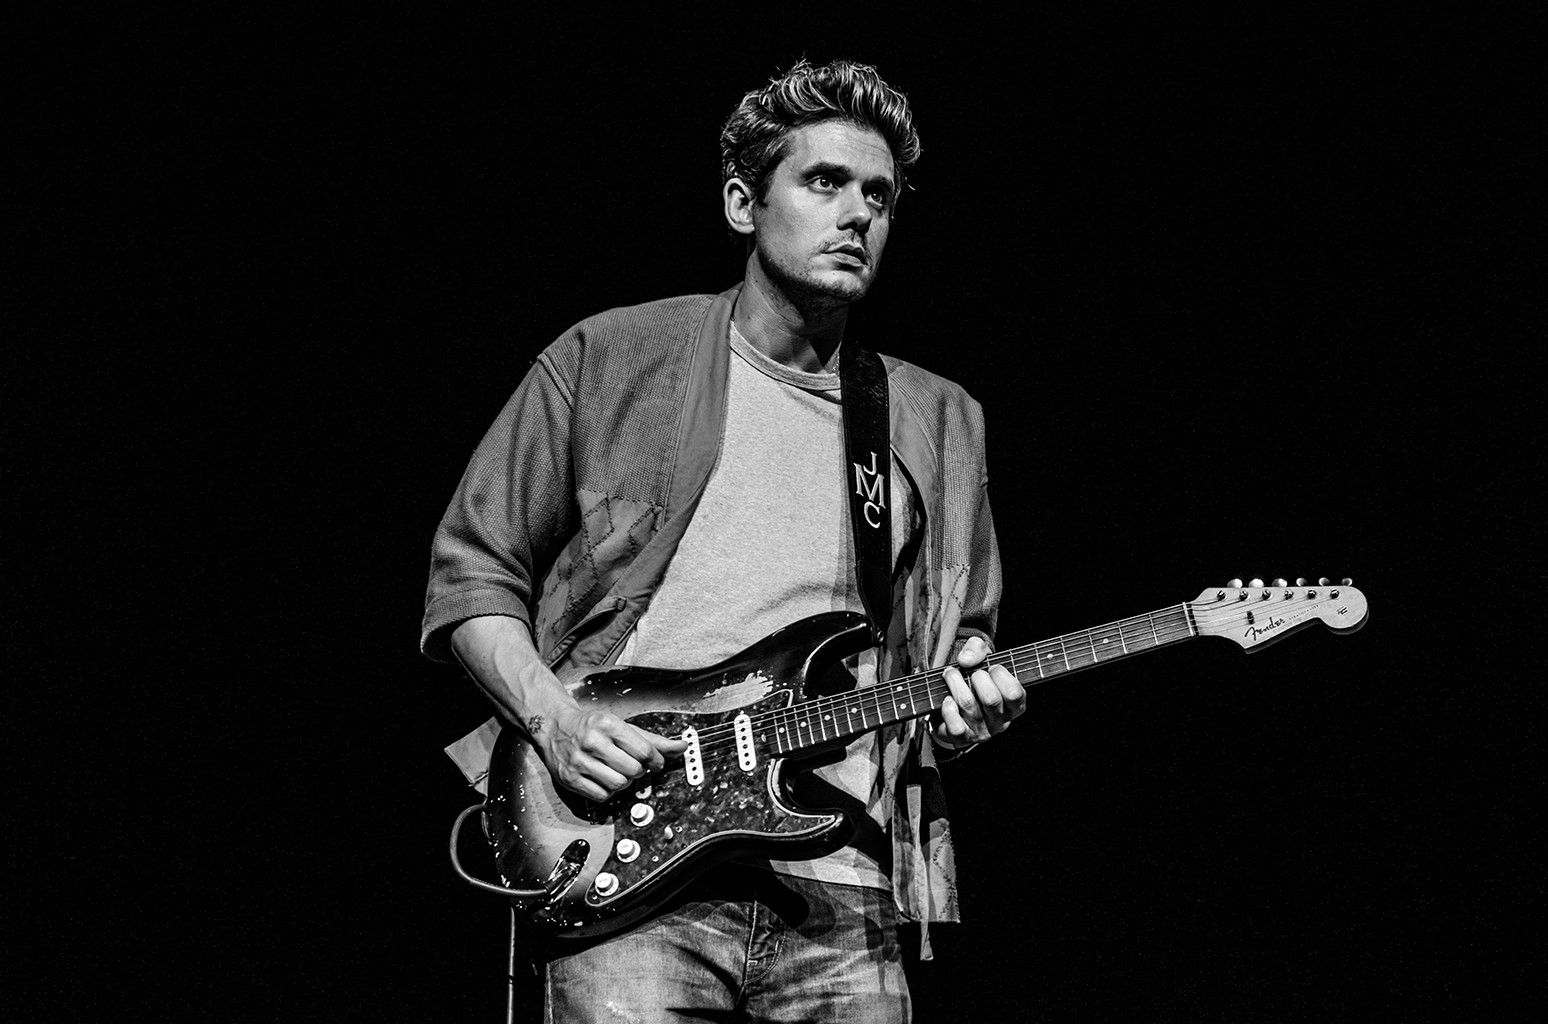
\includegraphics[width=\linewidth]{author/JM.jpg}
  \caption{COOOOOOOOOOOOOOOOOOOOOOL!!!!}
  \label{fig:3}
\end{figure}

\lipsum[4]

\subsection{Redow d asda}
\label{subsec:5}
\lipsum[4]
\cite[myjournal]{myjournal}
\lipsum[4]
